\documentclass[a4j,12pt]{jreport}
%\documentclass{jreport}
\usepackage[dvipdfmx]{graphicx}
% \usepackage[dvipdfmx]{graphics}
\usepackage{amsmath,amssymb}
% \usepackage{amsmath}
%\usepackage{pxjahyper}
\usepackage{here}
\usepackage{algorithm}
\usepackage{algpseudocode}
\usepackage{hhline} 
\usepackage[hang,small,bf]{caption}
\usepackage[subrefformat=parens]{subcaption}
\usepackage{url}
\usepackage{bm}
\captionsetup{compatibility=false}

\def\syaji{ \chapter*{謝辞} \addcontentsline{toc}{chapter}{謝辞}}
\renewcommand{\bibname}{参考文献}
\setlength{\textheight}{\paperheight}
\setlength{\topmargin}{4.6mm}
\addtolength{\topmargin}{-\headheight}
\addtolength{\topmargin}{-\headsep}
\addtolength{\topmargin}{-\headheight}
\addtolength{\textheight}{-60mm}

\setlength{\textwidth}{\paperwidth}
\setlength{\oddsidemargin}{-0.4mm}
\setlength{\evensidemargin}{-0.4mm}
\addtolength{\textwidth}{-50mm}

\begin{document}

%%%%%%%%%%%%%%%%%%%%%
% 表紙
%%%%%%%%%%%%%%%%%%%%%
\thispagestyle{empty}
\begin{center}
\begin{Large}
\vspace*{0.7cm}
{\large 中央大学大学院理工学研究科情報工学専攻\\修士論文}\\
\vspace*{2.5cm}
{\LARGE\bf 煙シミュレーションのための部分空間法の高速化}\\
\vspace*{0.7cm}
{\sf Accelerated Subspace Method for 3D Smoke Simulation}\\
\vspace*{6.5cm}
須之内 俊樹\\
Toshiki SUNOUCHI\\
学籍番号\hspace*{1zw}23N8100018B\\
\vspace*{2.5cm}
指導教員\hspace*{1zw} 森口 昌樹 准教授\\
\vspace*{2.5cm}
2025年3月\\
\end{Large}
\end{center}


%%%%%%%%%%%%%%%%%%%%%
% 概要
%%%%%%%%%%%%%%%%%%%%%
\newpage
\renewcommand{\baselinestretch}{1.25} \selectfont
\pagenumbering{roman}


\begin{center} {\large \bf{概 要}} \end{center}

\vspace{1zw} \noindent
{\bf キーワード: }流体シミュレーション,部分空間法,Snapshot 固有直交分解,Cubature

%%%%%%%%%%%%%%%%%%%%%
% 目次
%%%%%%%%%%%%%%%%%%%%%
\tableofcontents


\newpage
\pagenumbering{arabic}

%%%%%%%%%%%%%%%%%%%%%
% 1章
%%%%%%%%%%%%%%%%%%%%%
\chapter{序論} \label{chapter:1}

流体シミュレーションとは,コンピュータを用いて,流体の位置,速度,圧力などの物理量を計算するものである.表現できる流体は,空気,ガスなどの気体や,水,土砂の混ざった水,蜂蜜のような粘性がある液体,砂粒などの固体の粒など多岐にわたる.また,2次元と3次元を扱うことができる.2次元では,水面に広がる波紋や,異なる流体が作り出すマーブル模様などがシミュレーションでき,3次元では私たちの身の回りの現象を広くシミュレーションすることができる.計算した結果を人間が見やすいように可視化することで,流体力学の理論だけでは把握することが困難な,空間に広がる流体の物理量の分布を把握することができるようになる.

流体シミュレーションは,工学分野とコンピュータグラフィックの分野で活用されている.工学分野では,流体に触れる製品の設計・開発において,製品と流体の相互関係を事前にシミュレーションすることで,実験のコスト削減などに役立っている.コンピュータグラフィックスの分野では,水や煙のそれらしいアニメーションを生成し,映像作品やゲームの演出に役立っている.コンピュータグラフィックスの分野では,現実の物理現象に忠実な計算よりも,それらしい振る舞いを高速に計算することや,ユーザーが表現を操作しやすいことが重要視されている.

近代的な高解像度の流体表現は計算負荷が高く,高速化の研究が盛んに行われている.コンピュータグラフィックスの分野における高速化において,大規模並列計算手法の適用性が重要視されている.流体シミュレーションの計算はGPUによる高速化と相性が良く,高速化手法もGPUに適用できるものが望まれている.
また,前処理によってシミュレーション計算に利用する行列の次元を削減し計算負荷を削減する,部分空間法が存在する.これらの手法はシミュレーション計算は高速に行うことができるが,前処理の計算負荷や空間計算量が大きいことに注意が必要である.

本研究では,部分空間法の計算負荷削減により,前処理にかかる時間の短縮を目指す.
	%\section{流体シミュレーションの活用}
	%\section{流体シミュレーションの課題}
	%\section{流体シミュレーションの高速化手法}
	%	\subsection{大規模並列計算}
	%	\subsection{部分空間法を用いた次元削減}
	%\section{本研究の目的}
%%%%%%%%%%%%%%%%%%%%%
% 2章
%%%%%%%%%%%%%%%%%%%%%
\chapter{関連研究} \label{chapter:2}
	%\section{ナビエ・ストークス方程式}
	%\section{計算手法}
	\section{流体シミュレーション}
		%\subsection{ナビエ・ストークス方程式}
		%\subsection{離散化手法}
		%\subsection{Semi-Lagragian法を用いた移流項計算}
		%\subsection{Corinの射影法を用いた圧力項計算}
		%\subsection{気体らしい外力項計算}
		
		まず,流体シミュレーションの分野で一般的に使われている表記の説明をする.
		\begin{quote}
		\begin{itemize}
		\item $\bm{x}:$ 流体の位置を表すベクトル.シミュレーションする空間によって2次元,または3次元になる.
		\item $t:$ 時刻を表す変数.シミュレーション開始の時刻を$0$とする.
		\item $\varDelta x,\varDelta t:$ 離散化する計算格子の格子幅,次の時刻までの時間幅.
		\item $\bm{u} (\bm{x},t) :$ 位置$\bm{x}$,時刻$t$での流体の速度ベクトル.
		\item $p (\bm{x},t) :$ 位置$\bm{x}$,時刻$t$での流体の圧力値.
		\item $\rho,\nu:$ それぞれ,流体の密度,流体の粘性.ここでは位置や時刻によらない定数とする.
		\item $\bm{f}:$ 位置$\bm{x}$,時刻$t$での流体にかかる外力ベクトル.重力などはここに含める.シミュレーションの手法によっては外力を位置$\bm{x}$,時刻$t$によって変化する外力を扱うことができるが,今回は簡単のため,重力のみを扱い,どの位置でも,どの時刻でも一定の値として考える.
		\item $\nabla:$ 空間微分演算子ナブラ.スカラー場に作用させると勾配を表し,ベクトル場に作用させると発散を表す.3次元空間なので,$\nabla=  (\frac{\partial}{\partial x},\frac{\partial}{\partial y},\frac{\partial}{\partial z}) $ 
		\item $\frac{\rm{D}}{\rm{D}t} =\frac{\partial}{\partial t} + \bm{u} (\bm{x},t)  \boldsymbol{\cdot}\nabla$ :
		ラグランジュ微分,または物質微分.流体力学のような,連続体を扱う力学で用いられており,流れに沿って移動する物体と同じように移動する観測者から見た,物理量の時間変化率を表している.
	\end{itemize}
	\end{quote}

	下記の式\ref{eq:Navie}で表される式を,ナビエ・ストークス方程式とよび,これは流体力学の支配方程式である.非線形二階微分方程式となっており,代数的に一般解を求める事ができない.
	下記の式\ref{eq:compressed}は流体の連続の式と呼ばれる,質量保存や流量保存を表す式である.水や砂粒のように圧縮されない流体を扱うときは,流体の密度が常に一定,つまり密度の時間微分が0になり,それに伴い式\ref{eq:compressed}の左辺の第二項も0になる.これにより,式\ref{eq:uncompressed1}と,式 \ref{eq:uncompressed} を得る.式 \ref{eq:Navie} と式\ref{eq:uncompressed} または式 \ref{eq:uncompressed1}を連立することで非圧縮性流体の速度を求めることができる.ナビエ・ストークス方程式を扱う際は,コンピューターで近似解を解析的に求める手法が用いられる.
	
	\begin{equation}\label{eq:Navie}
		\frac{\partial}{\partial t}\bm{u} (\bm{x},t)  = - (\bm{u} (\bm{x},t)  \boldsymbol{\cdot}\nabla) \bm{u} (\bm{x},t)   - \frac{1}{\rho}\nabla p (\bm{x},t)  + \nu\nabla^2\bm{u} (\bm{x},t)  + \bm{f}
	\end{equation}
	\begin{equation}\label{eq:compressed}
		\frac{\rm{D}}{\rm{Dt}}\rho + \nabla\boldsymbol{\cdot}\bm{u} (\bm{x},t)  = 0
	\end{equation}
	\begin{equation}\label{eq:uncompressed1}
		\frac{\rm{D}}{\rm{Dt}}\rho  = 0
	\end{equation}
	\begin{equation}\label{eq:uncompressed}
		\nabla\boldsymbol{\cdot}\bm{u} (\bm{x},t)  = 0
	\end{equation}

%移流項は非線形であり,その他は線形である.
一般の非線形微分方程式は厳密な解析的解法が存在せず,様々な条件を設定した上で,数値解法により離散化し,近似解を求めるのが一般的である.ナビエ・ストークス方程式の数値解法は,中間の速度$\bm{u^*_i} (\bm{x},t)$を用いて,右辺の項について個別に方程式の近似解を求める手法が一般的である.式 (\ref{eq:Navie}) の右辺の第一項を移流項,第二項を圧力項,第三項を粘性項,第四項を外力項とよぶ.

Losassoらが提案したMarker And Cell法 (MAC法) \cite{MAC}と呼ばれる手法は,時間微分の離散化に前進差分を用いてナビエストークス方程式の数値解を求める代表的な手法である.MAC法は仮の速度$\bm{u}^*$を用いてナビエ・ストークス方程式を分割し,それぞれ個別に計算を行う.
\begin{equation}
	\bm{u} (\bm{x},t + \varDelta t)  =  \bm{u}^* - \varDelta t (\frac{1}{\rho}\nabla p (\bm{x},t)  + \nu\nabla^2\bm{u} (\bm{x},t)  + \bm{f}) 
\end{equation} 

\begin{equation}
	\bm{u}^* = \bm{u} (\bm{x},t)  - \varDelta t (\bm{u} (\bm{x},t)  \boldsymbol{\cdot}\nabla) \bm{u} (\bm{x},t)  
\end{equation}

ナビエストークス方程式の空間の離散化については,大きく分けて格子法(Eulerian)と粒子法(Lagrangian)がある.
格子法とは,流体を扱う空間を正方形や立方体の格子に区切り,格子の中心や辺,頂点などに物理量を配置して計算する方法である.区切る格子の数が多いほど,流体の詳細な動きが計算できるが,計算負荷は増加する.格子法の利点は,規則正しく並んだ格子で空間を離散化することで,微分演算を差分法などの方法で近似することができることや,境界条件の設定が容易であることが挙げられる.一方で,格子法の欠点は,格子の大きさよりも細かい表現が正確に行えないことや,格子内の流体の粒子の運動を平均化することにより,個々の粒子の詳細な運動を追跡することができないことが挙げられる.これらの欠点により,薄く広がった流体の運動や,水飛沫などを表現することが困難である.

粒子法は,流体の粒子の運動を追跡する手法であり,薄く広がった流体の運動や水飛沫などを表現することが容易である利点がある一方で,計算精度の保証が不十分であることや,境界条件の設定が煩雑になるという欠点がある.

格子法と粒子法は固体にも適用することが可能であり,流体とは異なる支配方程式を用いて変形や移動を計算することができる.流体と固体の相互関係をシミュレーションする際は,格子法と粒子法をそれぞれ個別に適用することが可能である.また,流体の移流項のみを粒子法を用いて計算し,そのほかを格子法で計算するなど,各項の計算について個別に適用する手法が存在する.
%微分計算の差分近似によって,無視されてしまう項が存在する.格子法での移流項の計算に用いられる差分近似で無視される項を,数値拡散,または人工粘性と呼ぶ.格子法での移流項の計算には風上差分がよく用いられるが,簡単のため,前進差分を用いる.格子法の欠点は,この数値拡散が決して小さくないため,移流項の精度があまりよくないことである.しかし,以下の移流項の計算によって,移流項の数値拡散として粘性項に似た形の式が現れる.従って,粘性項は移流項の数値拡散として扱い,まとめて計算されることが多い.また,水飛沫などの,液体が細かく分散するような計算は困難である.これは,微分の計算を差分で近似することで,隣接する格子との相互関係を用いて計算することになるため,液体が分散すると計算がうまくいかないためである.


\section{部分空間法}
	部分空間法は,ベクトル空間をより低次元の部分空間に射影し,数値シミュレーションにおける計算負荷を軽減する手法である.流体シミュレーションにおける部分空間法は,モデル縮約やモデル縮退とも呼ばれている.扱うベクトルデータやシミュレーションの計算を低次元の部分空間に射影して行い計算負荷を軽減する.以下では,部分空間法の理論の概要を説明する.
	
	シミュレーションの前処理として,$n$次元ベクトル$\bm{x}$を$r$次元ベクトル$\bm{y}$に変換する,$n \times r$直交行列$\mathbf{A}$を考える.以下の2式が成り立つ.
 	\[
 		\bm{y} = \mathbf{A^T}\bm{x}
 	\]
	\[
		\bm{x} = \mathbf{A}\bm{y}
	\]	
	また,$\bm{y'} = \mathbf{A^T}\bm{x'}$を満たす$n$次元ベクトル$\bm{x'}$,$r$次元ベクトル$\bm{y'}$について,以下の2式が成り立つような,任意の$m \times n$行列$\mathbf{F}$,任意の$m \times r$行列$\mathbf{\tilde{F}}$を考える.
	\[
		\bm{x'} = \mathbf{F}\bm{x}
	\]
	\[
		\bm{y'} = \mathbf{\tilde{F}}\bm{y}
	\]
$\bm{y'} = \mathbf{A^T}\bm{x'}$に,$\bm{x'} = \mathbf{F}\bm{x}$と,$\bm{x} = \mathbf{A}\bm{y}$を代入することで,
	\[
		\bm{y'} = (\mathbf{A^T}\mathbf{F}\mathbf{A})\bm{y}
	\]
	が得られる.$\bm{y'} = \mathbf{\tilde{F}}\bm{y}$と比較すると,
	\[
	\mathbf{\tilde{F}} = \mathbf{A^T}\mathbf{F}\mathbf{A}
	\]
	が得られる.
	
	以上により,任意のベクトルに対する行列積を,$n \times r$直交行列$\mathbf{A}$を用いて部分空間に射影することができる.流体シミュレーションにおいて,部分空間に射影したベクトルを用いてシミュレーション計算をするためには,射影後のベクトルも流体の非圧縮性条件等の性質を満たさなければならない.そのような射影を達成する行列$\mathbf{A}$を得る手法として,Snapshot固有直交分解がある.行列$\mathbf{A}$を既存の流体のデータを主成分分析を用いて計算することで,流体の性質を満たした射影が可能である.以降はSnapshot固有直交分解の具体的な計算方法について説明する.
	
	時刻$t \{t \in N, 0 \le t \le m\}$の$n$次元ベクトルデータ$\bm{u_t}$を用いて,$n\times m$行列$\mathbf{S}$を定義する.
		 \[ \mathbf{S} = 
        		\begin{bmatrix}
   | & | &  & |\\
   \bm{u}_0 & \bm{u}_1 &\cdots  & \bm{u}_{m-1} \\
   | & | &  & |
\end{bmatrix}
\]
	次に,行列$\mathbf{S}$主成分分析を行うため,$n \times r$行列$\mathbf{A}$について以下の最小化問題を考える.ここで$r$は抽出したい主成分の数である.
\[
min || \mathbf{S} -  \mathbf{A}\mathbf{A^T} \mathbf{S}||^2_F
\]


この最小化問題の解となる行列$\mathbf{A}$は,$\mathbf{S}\mathbf{S^T}$の固有ベクトル$\bm{v_i}(0 \le i \le r-1)$を用いて,以下の行列になる.
 \[ 
 \mathbf{A}  = 
        		\begin{bmatrix}
   | & | &  & |\\
   \bm{v}_0 & \bm{v}_1 &\cdots  & \bm{v}_{r-1} \\
   | & | &  & |
\end{bmatrix}
\]
ここで,固有ベクトル$\bm{v_i}$に対応する固有値を$\lambda_i$は,$\lambda_0 \ge \lambda_1 \cdots \ge \lambda_i \ge \lambda_{n-1} $を満たすとする.$\mathbf{S}\mathbf{S^T}$は対称行列になっているため,固有ベクトルは互いに直交し,$\mathbf{A^{-1}} = \mathbf{A^T}$となる.%また,$n \times n$行列$\mathbf{S^T}\mathbf{S}$ と$m\times m$行列$\mathbf{S}\mathbf{S^T}$の固有ベクトルは

次に,行列$\mathbf{A}$を用いて$\bm{u}$を$\bm{y}$に射影するとき,$\bm{y}$が流体の非圧縮性条件$\nabla\boldsymbol{\cdot}\bm{y} = 0$を満たしていることを確かめる.行列$\mathbf{S}$の各列ベクトル$\bm{u_i}$は既存のシミュレーションの速度データであるため,流体の非圧縮性条件$\nabla\boldsymbol{\cdot}\bm{u_i} = 0$を満たす.このことから,
\[
	\nabla\boldsymbol{\cdot}\mathbf{S}\ = \sum_{0 \le i \le n-1}\nabla\boldsymbol{\cdot}\bm{u_i} = 0
\]
が成り立つ.
行列$\mathbf{S}\mathbf{S^T}$の固有ベクトル$\bm{v_i}$と,それに対応する固有値を$\lambda_i$とすると,固有値と固有ベクトルの定義から以下が成り立つ.
\[
	\mathbf{S}\mathbf{S^T}\bm{v_i} = \lambda_i\bm{v_i}
\]
両辺に左から$\nabla\boldsymbol{\cdot}$を取ることにより,
	%\subsection{}
	%\section{ボリュームデータの可視化手法}
\chapter{煙の流体シミュレーション}
流体シミュレーションを行う際,境界条件や外力項を適切に設定することで,流体の振る舞いを操作することができる.この章では,部分空間法を用いて高速化するシミュレーションを実装する具体的な手法を紹介する.この手法で得られたシミュレーションデータを用いて,部分空間法に用いるSnapshot固有直交分解を行う.

\section{格子法による離散化}
格子法による空間の離散化は,扱う格子によって様々な手法が存在する.例えば物理量を格子の中心に配置するコロケート格子や,速度成分を格子の面の中心に配置するスタッガード格子が存在する.コロケート格子は流体の格子の形状によらず適用できるが,境界条件の設定が煩雑である.スタッガード格子は適用が立方体格子などに限定される一方,境界条件の設定が容易である.本論文では,シミュレーション空間をスタッガード格子を用いて離散化する.スタッガード格子は下記の図\ref{fig:staggerd}のように,格子の中心を圧力の位置に定義し,格子面の中心に,その格子面と垂直な流速の成分の位置を定義する.例えば$xy$平面に並行な格子面には,その地点での流速の$z$成分を配置する.
シミュレーション空間の$x$,$y$,$z$軸方向の分割数を$nx$,$ny$,$nz$とする.スタッガード格子によってシミュレーションの物理量を,以下のベクトルに離散化する.
\begin{itemize}
	\item	$\bm{v_x}$:$(nx+1) \times ny \times nz$次元ベクトル.
	\item	$\bm{v_y}$:$nx \times (ny+1) \times nz$次元ベクトル.
	\item	$\bm{v_z}$:$nx \times ny \times (nz+1)$次元ベクトル.
	\item $\bm{p}$:$nx \times ny \times nz$次元ベクトル.
\end{itemize}

$\bm{v_x}$,$\bm{v_y}$,$\bm{v_z}$は速度の$x$,$y$,$z$成分,$\bm{p}$は圧力である.
ここで,前進差分を用いた空間の偏微分の離散化の例として,スタッガード格子を用いた以下の偏微分の離散化を上記のベクトルを用いて表現することを考える.
\[
\frac{\partial}{\partial \bm{x}}\bm{u} (\bm{x}) = \frac{\bm{u}(\bm{x}+\varDelta \bm{x})  - \bm{u} (\bm{x}) }{\varDelta \bm{x}}
\]
ここで,$\bm{u} (\bm{x})$は位置$\bm{x}$での速度を表す三次元ベクトルである.
スタッガード格子の一辺の長さを$\varDelta L = \varDelta \bm{x}$,流体の位置ベクトル$\bm{x}$を自然数$i(0 \le i \le nx-1),j(0 \le j \le ny-1),k(0 \le k \le nz-1)を用いて,$$\bm{x} = (i\varDelta L,j\varDelta L,k\varDelta L)$とすると,以下のようになる.
\[
\frac{\bm{u}(\bm{x}+\varDelta \bm{x})  - \bm{u} (\bm{x}) }{\varDelta \bm{x}}
= \begin{bmatrix}
\frac{\bm{v_x}(i+1,j,k)  - \bm{v_x} (i,j,k) }{\varDelta L}\\
\frac{\bm{v_y}(i,j+1,k)  - \bm{v_y} (i,j,k) }{\varDelta L}\\
\frac{\bm{v_z}(i,j,k+1)  - \bm{v_z} (i,j,k) }{\varDelta L}
\end{bmatrix}
\]

このような離散化を用いて,以降は気体の流体シミュレーションにおけるナビエ・ストークス方程式の計算方法を説明する.
\begin{equation}\label{eq:linear}
	\bm{u} (\bm{x},t + \varDelta t)  =  \bm{u}^* - \varDelta t (\frac{1}{\rho}\nabla p (\bm{x},t)  + \nu\nabla^2\bm{u} (\bm{x},t)  + \bm{f}) 
\end{equation} 

\begin{equation}\label{eq:nonlinear}
	\bm{u}^* = \bm{u} (\bm{x},t)  - \varDelta t (\bm{u} (\bm{x},t)  \boldsymbol{\cdot}\nabla) \bm{u} (\bm{x},t)  
\end{equation}

上記の式\ref{eq:linear}と式\ref{eq:nonlinear}を以下のように各項ごとに分割して計算する.
\begin{equation}\label{eq:force}
	\bm{u_0(\bm{x})} =  \bm{u} (\bm{x},t)  - \varDelta t \bm{f} 
\end{equation} 

\begin{equation}\label{eq:advect}
	\bm{u_1(\bm{x})} = \bm{u_0(\bm{x})}  - \varDelta t (\bm{u_0} (\bm{x})  \boldsymbol{\cdot}\nabla) \bm{u_0} (\bm{x})
\end{equation}

\begin{equation}\label{eq:diffusion}
	\bm{u_2(\bm{x})}   =  \bm{u_1(\bm{x})} - \varDelta t \nu\nabla^2\bm{u_1} (\bm{x})
\end{equation}

\begin{equation}\label{eq:pressure}
	\bm{u} (\bm{x},t + \varDelta t)= \bm{u_3(\bm{x})}  =  \bm{u_2(\bm{x})} - \varDelta t (\frac{1}{\rho}\nabla p (\bm{x})
\end{equation} 

ここで,式\ref{eq:force}は外力項,式\ref{eq:advect}は移流項,式\ref{eq:diffusion}は粘性項,式\ref{eq:diffusion}は粘性項,式\ref{eq:pressure}は圧力項を計算する式であり,これらの両辺を全て足し合わせると元のナビエ・ストークス方程式が得られる.
\subsection{外力項計算}
\begin{equation}
	\bm{u_0} =  \bm{u} (\bm{x},t)  - \varDelta t \bm{f} 
\end{equation} 
外力項では,再現したい現象になるような外力を与えなければならない.コンピュータグラフィックスにおける気体の外力は,気体にかかる重力と,温度差による対流を発生させる力,気体が渦巻くように与える力などをユーザーがパラメータによって調整できるようにする計算方法が一般的である.よりそれらしい振る舞いを再現するため,他の計算では定数として扱う密度や温度を,ここでは位置と時刻によって変化するデータとして計算する.
位置$\bm{x}$における気体の密度,温度をそれぞれ$\rho(\bm{x})$,$T(\bm{x})$とし,
\section{ボリュームデータの可視化手法}

\chapter{部分空間法} \label{chapter:3}
	\section{基底空間構築手法}
	\section{流体ソルバへの部分空間法の適用}
		%\subsection{テンソルを用いた線形項の次元削減}
		%\subsection{Cubature法を用いた非線形項の次元削減}
	\section{部分空間法の課題}
	
\chapter{部分空間法の高速化手法の提案} \label{chapter:3}
	\section{Snapshotの分割による高速化}
	\section{領域分割による高速化}
	\section{計算機実験}
		\subsection{計算条件}
		\subsection{計算結果}
	\section{課題}
\chapter{結論}

%計算機が登場する以前の流体力学は,実際の流体を用いて実験を繰り返さなければならなかったが,計算機が登場してからは,シミュレーションをすることで,計算機上で流体の振る舞いを確認できるようになった.計算機を使った流体力学を特別に,数値流体力学 (CFD: Computational Fluid Dynamics) と呼び分けることも多い.CFDは実験で得ることが困難な,流れ場全体の詳細な情報を得ることができる.CFDは流体に触れる製品の設計・開発に非常に大きな貢献をした.

%また,コンピューターグラフィックスにおいても,流体のアニメーションを計算することができるCFDが貢献していて,映像作品やゲームなどで利用されている.コンピューターグラフィックスにおいては,それらしい流体の運動がリアルタイムでシミュレーションできることが重要視される.精度良く計算できることはそこまで重要視されておらず,場合によってはそれらしさのために,現実より大袈裟なシミュレーションをすることもある.

%\section{基礎概念}
%数値流体力学では,シミュレーションする空間を離散化して計算を行う.離散化は,各辺が空間の座標軸に並行な計算格子を用いて空間を分割する.この計算格子上に物理量を定義して計算を行う.どのように定義して計算を行うかは手法によって異なる.ある時刻で空間の物理量の分布を計算した後,時刻を時間の刻み幅分進めて,次の時刻の計算をすることを繰り返してシミュレーションを行う.
%\subsection{ナビエ・ストークス方程式} \label{subsec:nabie}


%\subsubsection{格子法における移流項の計算} \label{subsec:gridadvect}
\begin{equation}\label{eq:uncalculated_pressure_before}
\frac{\partial}{\partial t}\bm{u} (\bm{x},t)  = -\bm{u} (\bm{x},t) \frac{\partial}{\partial \bm{x}}\bm{u} (\bm{x},t)
\end{equation} 

%偏微分演算子を前進差分$\frac{\partial}{\partial \bm{x}}\bm{u} (\bm{x},t)  = \frac{\bm{u} (\bm{x}+\varDelta \bm{x},t)  - \bm{u} (\bm{x},t) }{\varDelta \bm{x}}$を用いて離散化すると,
%$$\frac{\partial}{\partial t}\bm{u} (\bm{x},t)  =  -\bm{u} (\bm{x},t) \frac{\bm{u} (\bm{x}+\varDelta \bm{x},t)  - \bm{u} (\bm{x},t) }{\varDelta \bm{x}}$$
%が得られる.
%二変数のテーラー展開$f (a+h,b+k)  \fallingdotseq \sum\limits_{t=0}^n \frac{1}{t!} (h\frac{\partial}{\partial \bm{x}} + k\frac{\partial}{\partial y}) ^t f (a,b) $を二次まで行い,式を整理すると,
%$$\frac{\partial}{\partial t}\bm{u} (\bm{x},t)  = -\frac{1}{2!\varDelta \bm{x}}\bm{u} (\bm{x},t) \left (  (\bm{u} (\bm{x},t) +\varDelta t\frac{\partial}{\partial \bm{x}}\bm{u} (\bm{x},t)  +  (\varDelta \bm{x}) ^2\frac{\partial^2}{\partial \bm{x}^2}\bm{u} (\bm{x},t)  \right) $$
            
%$$\frac{\partial}{\partial t}\bm{u} (\bm{x},t)  =  -\bm{u} (\bm{x},t) \left (\frac{\partial}{\partial \bm{x}}\bm{u} (\bm{x},t)  + \varDelta \bm{x}\frac{\partial^2}{\partial \bm{x}^2}\bm{u} (\bm{x},t)  \right) $$

%$$ \frac{\partial}{\partial t}\bm{u} (\bm{x},t)  =  -\bm{u} (\bm{x},t) \frac{\partial}{\partial \bm{x}}\bm{u} (\bm{x},t)  -\bm{u} (\bm{x},t) \varDelta \bm{x}\frac{\partial^2}{\partial \bm{x}^2}\bm{u} (\bm{x},t) $$

%が得られる.ここで,$ -\bm{u} (\bm{x},t) \varDelta \bm{x} = \mu$とし,$\frac{\partial^2}{\partial \bm{x}^2}\bm{u} (\bm{x},t)  = \nabla^2\bm{u} (\bm{x},t) $とすれば,
%\frac{\partial}{\partial t}\bm{u} (\bm{x},t)  =  -\bm{u} (\bm{x},t) \frac{\partial}{\partial \bm{x}}\bm{u} (\bm{x},t)  +\mu\nabla^2\bm{u} (\bm{x},t) ) 
%\end{equation} 
%が得られる.式( \ref{eq:uncalculated_pressure_before}) と式( \ref{eq:uncalculated_pressure_before}) を比較すると,右辺の二項目が数値拡散であること,そして数値拡散は粘性項の式とよく似ていることがわかる.
\subsubsection{格子法における非線形項の計算} \label{subsec:gridpressure}
式 (\ref{eq:linear}) の粘性項は先述の通り省略し,外力項は事前に流速に与えて扱うことができるため省略する.残った圧力項の計算について考える.ただし,移流項を先に計算し,$\bm{u}^*$は既知のものとする.
\begin{equation}\label{eq:uncalculated_pressure}
\bm{u} (\bm{x},t+1)  =  \bm{u}^* - \frac{\varDelta t}{\rho}\nabla p (\bm{x},t) 
\end{equation} 
両辺の発散をとると,
$$\nabla\boldsymbol{\cdot}\bm{u} (\bm{x},t+1)  =  \nabla\boldsymbol{\cdot}\bm{u}^* - \frac{\varDelta t}{\rho}\nabla^2 p (\bm{x},t) $$
が得られ,流体の非圧縮性条件,$\nabla\boldsymbol{\cdot}\bm{u} (\bm{x},t)  = 0$により,左辺は0になるため,
\begin{equation}\label{eq:calculated_pressure}
\nabla\boldsymbol{\cdot}\bm{u}^* = \frac{\varDelta t}{\rho}\nabla^2 p (\bm{x},t) 
\end{equation} 
が得られる.この式を満たすような圧力を求め,上記の式 (\ref{eq:uncalculated_pressure}) に代入することによって,次の時刻の流速$\bm{u} (\bm{x},t+1) $が計算できる.式 (\ref{eq:calculated_pressure}) のような微分方程式はポアソン方程式と呼ばれ,境界条件として,扱う領域の境界での$p (\bm{x},t) $の値を計算前に定めることで,式を満たすような変数を求めることができる.
%\subsubsection{格子法における物理量の位置の定義方法} \label{subsec:grid_sampling}
\begin{figure}[htbp]
\begin{center}
%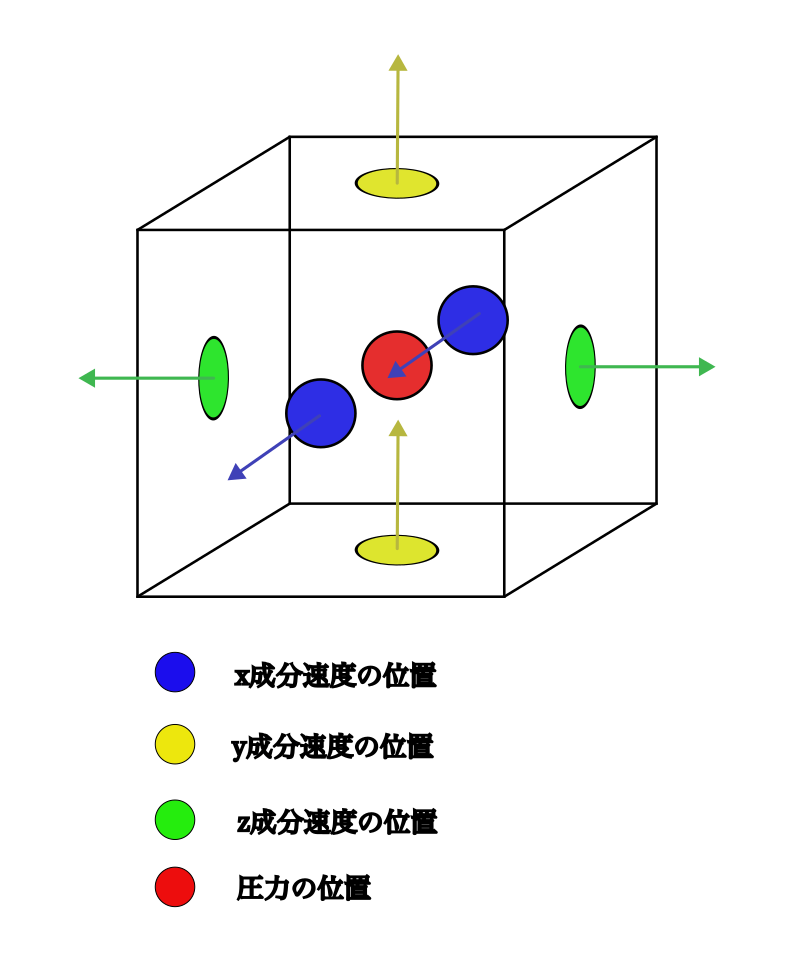
\includegraphics[width=80mm]{3dstaggerd.png}
\caption{スタッガード格子}
\label{fig:staggerd}
\end{center}
\end{figure}.

%\subsubsection{スタッガード格子を用いた,格子法の線形項の計算の離散化方法}
\begin{figure}[htbp]
\begin{center}
%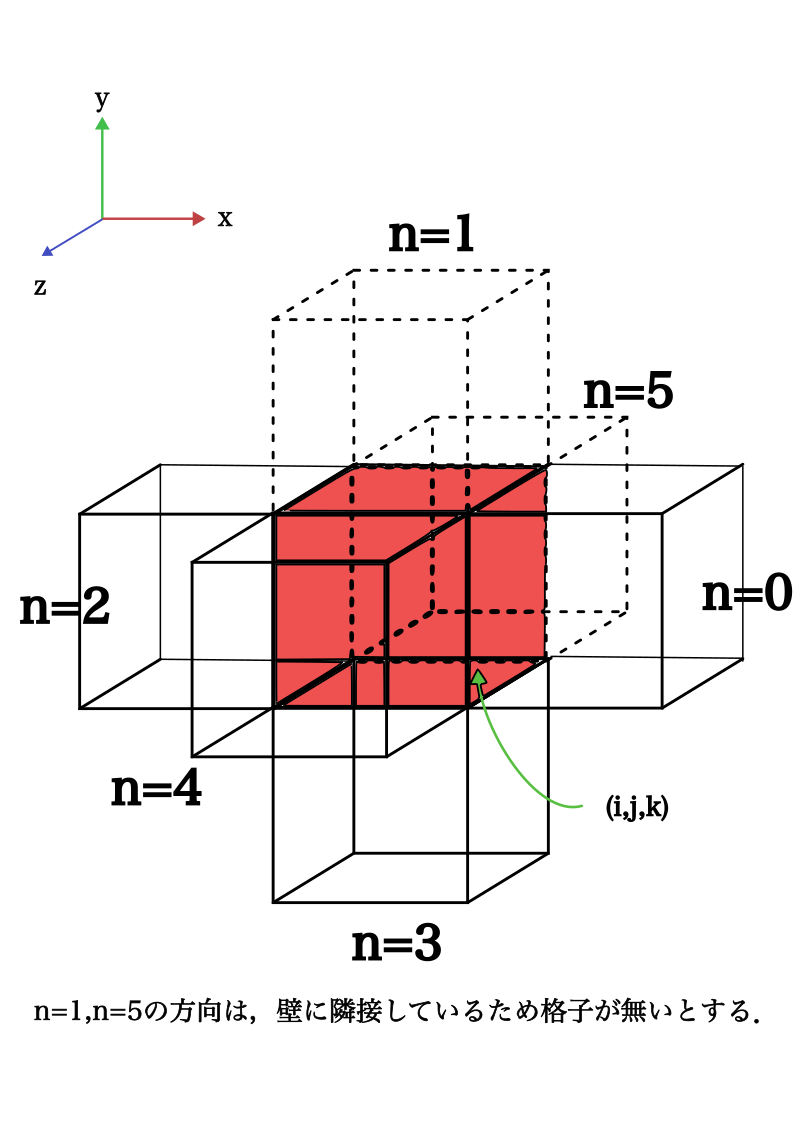
\includegraphics[width=80mm]{pressure_model.png}
\caption{圧力計算のモデル}
\label{fig:pressure_model}
\end{center}
\end{figure}
圧力項の計算を,スタッガード格子を用いて離散化するため,先ほどの式 (\ref{eq:calculated_pressure}) を考える.
$$\nabla\boldsymbol{\cdot}\bm{u}^* = \frac{\varDelta t}{\rho}\nabla^2 p (\bm{x},t) $$
スタッガード格子では圧力と流速が配置してある位置がずれている.従って,空間微分に対して同じ差分を適用すると,同じ幅で差分を取ったとしても離散化される空間の位置がずれてしまうため,空間微分に対して同じ差分は適応できない.そこで差分を取るのではなく,両辺をセルの領域で積分して考える.
$$\int_V\nabla\boldsymbol{\cdot}\bm{u}^* dV= \int_V\frac{\varDelta t}{\rho}\nabla^2 p (\bm{x},t) dV$$
両辺にガウスの発散定理を適用すると,周回積分の形で表せる.
$$\oint_V\bm{u}^*\boldsymbol{\cdot}\bm{n} dV= \oint_V\frac{\varDelta t}{\rho}\nabla p (\bm{x},t) \boldsymbol{\cdot}\bm{n}dV$$
この式はスタッガード格子において,周回積分は格子の各面で境界条件を考えて,全ての面の物理量を足すことで表すことができる.
ここで離散化のため,$x軸方向にi番目,y軸方向にj番目,z軸方向にk番目の格子をg_{i,j,k},g_{i,j,k}の圧力をp_{i,j,k}と定義し,$図\ref{fig:pressure_model}のようなモデルを考える.

まず,整数$n=0,1,2,\cdots 5$までを,それぞれ格子の各面の方向に割り振る.図\ref{fig:pressure_model}の場合,$n=0$は$x$軸正の方向,$n=1$は$y$軸正の方向,$n=2$は$x$軸負の方向,$n=3$は$y$軸負の方向,$n=4$は$z$軸正の方向,$n=5$は$z$軸負の方向に割り振る.ここで,この整数$n$を使って,いくつかの配列や変数を定義する.
\begin{quote}
	\begin{itemize}
		\item $F_n$ 格子の面の各方向に隣接しているものが流体なら$1$,壁面なら$0$を取るブーリアン値.
		
		図\ref{fig:pressure_model}の場合,$n=0$に対応する$x$軸正の方向と,$n=5$に対応する$z$軸負の方向は壁に隣接していて格子がないため,$F_0,F_5 = 0,F_1,F_2,F_3,F_4 = 1$となる.
		\item $D_n$ 格子の面の各方向に垂直で,格子の外側を向く単位ベクトルを表す係数.向いている方向が座標軸の正の向きなら+1,					負の向きなら$-1$を取る整数値.
		
		図\ref{fig:pressure_model}の場合,座標軸の正の方向に向いているのは$n=0,n=1,n=4$に対応する方向で,それ以外は負の方向に向いているため,
		$F_0,F_1,F_4 = 1,F_2,F_3,F_4 = -1$となる.
		\item $p_n$ 割り振られた方向に隣り合っている格子の圧力値.
		図\ref{fig:pressure_model}の場合,$p_0 = p_{i+1,j,k}$,$p_1 = p_{i,j+1,k}$,$p_2 = p_{i-1,j,k}$,$p_3 = p_{i,j-1,k}$,$p_4 = p_{i,j,k+1}$,$p_5 = p_{i,j,k-1}$となるが,境界条件を考えると,壁に隣接している格子との圧力値の勾配を$0$にするため,$p_0 = p_{i,j,k}$,$p_5 = p_{i,j,k}$である.
		\item $\nabla\bm{p_n}$ 割り振られた方向の圧力勾配.前方差分によって,$\nabla \bm{p_n} (\bm{x},t)  = \frac{p_n - p_{i,j,k}}{\varDelta x}$と近似できる.
		\item $u_n$ $g_{i,j,k}$に配置されている流速値で,割り振られた方向の格子面に配置されている流速値.壁に隣接している方向は流速を$0$にするため,$u_0 = 0$,$u_5 = 0$である.
	\end{itemize}
\end{quote}

定義した配列や変数を用いて,周回積分の形で表された式を離散化することで,
$$ \sum_{n}\bm{u_n}^*D_nF_n\varDelta x = \sum_{n}\frac{\varDelta t}{\rho}\nabla p_n (\bm{x},t) F_n\varDelta x $$
が得られ,圧力勾配を$\nabla p_n (\bm{x},t)  = \frac{p_n - p_{i,j,k}}{\varDelta x}$で近似すると,

$$ \sum_{n}\bm{u_n}^*D_nF_n\varDelta x = \sum_{n}\frac{\varDelta t}{\rho}\frac{p_n (\bm{x},t) - p_{i,j,k} (\bm{x},t) }{\varDelta \bm{x}}F_n\varDelta x $$
が得られる.この式を整理すると,
\begin{equation}\label{eq:discretized_pressure}
\sum_{n}\bm{u_n}^*D_nF_n= \sum_{n}\frac{\varDelta t}{\rho}\frac{p_n (\bm{x},t)  - p_{i,j,k} (\bm{x},t) }{\varDelta \bm{x}}F_n
\end{equation} 
が得られる.
式 (\ref{eq:discretized_pressure}) は$p$についての連立一次方程式となっている.全ての格子に対して式 (\ref{eq:discretized_pressure}) を考えることになるため,連立方程式は規模が大きくなる.従って,直接法ではなく反復法を用いて,必要な精度で計算を打ち切って計算する.連立方程式の解法としては,前処理付き共役勾配法がよく用いられている.

%\subsubsection{ディリクレ境界条件} \label{subsec:Dirichlet}
圧力項の計算を離散化した式 (\ref{eq:discretized_pressure}) は,求めたい圧力分布の式 (\ref{eq:uncalculated_pressure}) を満たすような解が得られるが,得られた解がシミュレーション内で,良い圧力として振る舞うかどうかは考えなければならない.ディリクレ境界条件は,扱う領域を流体と気体の領域に分割し,流体の物理量のみを考える際に用いる境界条件で,流体が存在しない格子の圧力値を$0$とする.ディリクレ境界条件を考えずに流体の圧力のみを計算すると,気体の領域とされている場所にも流体の圧力が計算できてしまう.そのため,気体と液体の領域に分割するようなシミュレーションで,気体の圧力が液体の圧力に及ぼす影響が小さい場合は,圧力にディリクレ境界条件を追加した方が,より良い圧力分布になると言える.

%\subsection{粒子法} \label{subsec:particle}
粒子法とは,流体をいくつかの小さな粒子の集まりとして考え,各粒子に物理量を与えて計算をする方法である.本来は流体は,アボガドロ数 ($N_A = 6.02*10^{23}$) 単位の分子が動いているが,これら全てを計算機で扱うのは現実的でないため,いくつかの分子の動きを一つの粒子にまとめて扱う.粒子の数が多いほど実際の現象に近づき,精度が良くなるが,計算負荷は増加する.利点として,以下の計算によって,移流項の計算に数値拡散が発生しないことが確認できるため,移流項が精度良く計算できる.また,格子法では水飛沫の表現が困難であるが,粒子法は粒子が存在する場所に液体が存在すると考えるため,粒が飛び散りさへすれば水飛沫のような表現になる.欠点として,粒子が飛び散ったときに粒子の影響範囲内に他の粒子がいないとき,計算がうまくできないことから,正確な物理量の分布が計算できる訳ではない.また,対象の流体以外は計算しないことが多いため,例えば水と空気が入り混じるようなシミュレーションを考える際,水の計算のみをすることで,空気の影響が無視されてしまう.
%\subsubsection{粒子法における移流項の計算} \label{subsec:particleadvect}
簡単のため,ナビエストークス方程式から粘性項と外力項を取り除いた,オイラー方程式と呼ばれるものについて考える.
$$\frac{\partial}{\partial t}\bm{u} (\bm{x},t)  = - (\bm{u} (\bm{x},t) \boldsymbol{\cdot}\nabla) \bm{u} (\bm{x},t)  - \frac{1}{\rho}\nabla \bm{p}$$
粒子法はラグランジュ微分を用いることで、移流項の計算が単純になる。
時刻$t_0$に位置$\bm{x_0}$にある流体の速度を$\bm{u} (\bm{x_0},t_0) $とする.$\varDelta t$秒後の位置は$\bm{x_0}+v (\bm{x_0},t_0) \varDelta t$になっているので,時刻$t_0+\varDelta t$の流体の速度は、$\bm{u} (\bm{x_0}+\bm{u} (\bm{x_0},t_0) \varDelta t,t_0+\varDelta t) $となる。この間の速度変化$\varDelta \bm{u}$をテイラー展開を用いて表すと,

$$ \varDelta \bm{u} = \bm{u} (\bm{x_0}+v\varDelta t,t_0+\varDelta t)  - \bm{u} (\bm{x_0},t_0)  = \frac{\partial \bm{u} (\bm{x_0},t_0) }{\partial \bm{x}}\bm{u} (\bm{x_0},t_0) \varDelta t + \frac{\partial \bm{u} (\bm{x_0},t_0) }{\partial t}\varDelta t$$

両辺を$\varDelta t$で割ると,
$$ \frac{\varDelta \bm{u}}{\varDelta t} = \frac{\partial \bm{u} (\bm{x_0},t_0) }{\partial \bm{x}}\bm{u} (\bm{x_0},t_0)  + \frac{\partial \bm{u} (\bm{x_0},t_0) }{\partial t}$$
$$ \frac{\varDelta \bm{u}}{\varDelta t} =  (\bm{u}\boldsymbol{\cdot}\nabla) \bm{u} + \frac{\partial \bm{u} (\bm{x_0},t_0) }{\partial t}$$

ラグランジュ微分,つまり,粒子を流れに沿って動かしたときの変化量が,オイラー方程式の移流項になっている.粒子法では,物理量をもった粒子自体を動かすだけで,移流項の計算をすることができる.

%\subsection{部分空間法} \label{subsec:subspace}


%\section{関連研究} \label{sec:reratedworks}


%\chapter{提案手法} \label{chapter:4}

%\section{圧力項の離散化と実装} \label{sec:Imppressure}
\begin{equation}
\sum_{n}\bm{u_n}^*D_nF_n= \sum_{n}\frac{\varDelta t}{\rho}\frac{\bm{p_n} (\bm{x},t)  - \bm{p_{i,j,k}} (\bm{x},t) }{\varDelta \bm{x}}F_n
\end{equation}

圧力項は圧力を変数とした,上記の連立方程式を解く.格子の総数を$n$とすると,全ての格子で連立方程式を考えるため,合計$n$本の連立方程式を解くことになる.そこで,$\bm{Ax=b}$に対応させたものを解く.$\bm{A}$,$\bm{b}$それぞれのサイズは,$\bm{A}$は$n \times n$であり,$\bm{b}$は$n$である.この際,3次元に分布する圧力をベクトルにうつす.具体的には,圧力の$ (i,j,k) $成分は,ベクトルの$iN_yN_z+jN_x+k$成分にうつす.また,$\bm{A}$の$ (iN_yN_z+jN_x+k,lN_yN_z+mN_x+n) $の成分には,位置$ (i,j,k) $の格子についての連立方程式の,圧力の$ (l,m,n) $成分にかかる係数を保存すれば良い.通常の行列のままだと空間計算量や時間計算量をが非常に大きくなってしまうが,$\bm{A}$のほとんどの成分は$0$であることを利用し,Eigenの疎行列ライブラリを用いることで,空間計算量や時間計算量を削減できる.連立方程式の解法は,未知数が多いため,直接法で計算するのは現実的ではない.反復法では,必要な精度に解が収束したら計算を打ち切るため,解の収束が速い方が望ましい.前処理をすることで解の収束が速くなるため,前処理付き共役勾配法を採用し,Eigenの前処理付き共役勾配法を計算する関数を用いて連立方程式を解く.$\bm{A}$と$\bm{b}$の各成分は以下のように計算する.
\begin{quote}
	\begin{itemize}
		\item $\bm{A}$,$\bm{b}$を初期化する.この際,$\bm{b}$の成分は全て0にしておく.
		\item 全粒子について,ディリクレ境界条件を考え,粒子が存在しない空間の圧力を$0$で固定する.これは,standerdgridの$ (i,j,k) $に格納されている粒子の数を見て,0なら$\bm{A}$の$ (iN_yN_z+jN_x+k,iN_yN_z+jN_x+k) $成分を1にして,処理を終了すれば良い.
		\item 粒子が入っていたセル$ (i,j,k) $について,式 (\ref{eq:discretized_pressure}) に従って係数を計算する.セル$ (i,j,k) $の周囲の6方向に格納されている流速について,シミュレーションの境界で,壁に隣接していない方向についての流速の周回積分を計算する.周回積分の値を,$\bm{b}$の$ (iN_yN_z+jN_x+k) $成分に代入する.
		\item セル (i,j,k) の周囲の6方向のセルについて,粒子が入っていないセルの方向,または,壁に隣接している方向なら疎行列には何もせず,それ以外なら疎行列の$iN_yN_z+jN_x+k$行の,それぞれの方向に対応した対応した成分に$\frac{\varDelta t}{\rho\varDelta x^2}$を代入する.
	\end{itemize}
\end{quote}
%\section{シミュレーション領域の定義} \label{sec:levelsetserface}
本手法では,シミュレーションは立方体の内部の領域内で行う.立方体の一辺の長さ$L$は,スタッガード格子の水平方向の数を$N$,スタッガード格子の一辺の長さを$dx$とすると,$L = Ndx$である.
8点$ (0,0,0) , (L,0,0) , (0,L,0) , (0,0,L) , (L,L,0) , (0,L,L) , (L,0,L) , (L,L,L) $を頂点とするような立方体の領域を扱うレベルセットサーフェス$\varphi (x,y) $を,以下のように定義する.
\begin{equation}\label{eq:levelsetserface}
\varphi (x,y,z) 
\begin{cases}
 (x,y,z)  & x \le0 , y \le 0,z \le 0,\\
 (L - x,y,z)  & L \le x , y \le 0,z \le 0,\\
 (x,L-y,z)  & x \le0 , L \le y,z \le 0,\\
 (L-x,L-y,z)  & L \le x , L \le y,z \le 0,\\
 (x,y,L-z)  & x \le0 , y \le 0,L \le z,\\
 (L - x,y,L-z)  & L \le x , y \le 0,L \le z,\\
 (x,L-y,L-z)  & x \le0 , L \le y,L \le z,\\
 (L-x,L-y,L-z)  & L \le x , L \le y,L \le z,\\
 (0,0)  & \rm{else}.\\
\end{cases}
\end{equation} 
このようにして定義されるレベルセットサーフェスは,粒子の座標を引数とし,シミュレーションする立方体から外に出ていた場合は,立方体の領域内に最短距離で戻すようなベクトルを返り値として返す.粒子に対して移流計算や粒子位置の補正を行うと,シミュレーション領域から粒子が出ていってしまうことがあるため,そのような計算を行った後に全粒子に対して領域内部に戻す処理を行う.

%\section{図と表の例} \label{section:figure_table}

図・表には通し番号と見出し(caption)を付け,本文中で当該の図・表に言及する.また,単位や目盛を正確に記す.
図のタイトルは図の下に,表のタイトルは表の上に書く.

例を図\ref{fig:logo}と表\ref{tab:results}に示す.
第\ref{chapter:2}章の図には図2.1, 図2.2, 図2.3,…のように番号が振られ,
第\ref{chapter:2}章の表には表2.1, 表2.2, 表2.3,…のように,図とは独立に番号が振られる.


\begin{figure}[b]
    \centering
    %
\includegraphics[scale=0.5]{images/logo_color.png}
    \caption{情報工学科のロゴ}
    \label{fig:logo}
  \end{figure}


\begin {table}[t]
    \centering
  \caption{表のタイトル}
  \label{tab:results}
  \begin {tabular}{ccc} \hline
     項目1 & 項目2 & 項目3 \\ \hline
    データ1 & データ2 & データ3 \\
    データ1 & データ2 & データ3 \\
    データ1 & データ2 & データ3 \\ \hline
  \end {tabular}
\end {table}


%\section{参考文献の書き方}

一例として,和文の著書\cite{suetake},和文の論文誌\cite{kusano},英文の編書\cite{fuortes},
英文の論文誌\cite{rice},国際会議\cite{guibas},修士論文\cite{chudai},電子雑誌\cite{iwama},Webページ\cite{IPSJ}を,
2ページの参考文献の節に載せる.{\em 参考文献には信頼性が高く,後世に残るものを載せるように注意せよ.}

書くべき情報は以下のとおりである.
\begin{itemize}
\item 和文の著書: 著者,書名,シリーズ名(あれば),発行所,都市,年.
\item 和文の論文誌: 著者,題名,誌名,巻,号,頁,年.
\item 英文の編書: 編者,書名,発行所,都市,年.
\item 英文の論文誌: 著者,題名,誌名,巻,号,頁,年.
\item 国際会議: 著者,題名,予稿集名,都市,コード等,頁,年.
\item 修士論文: 著者,題名,機関名,年.
\item 電子雑誌: 著者,題名,誌名,巻,号,頁(オンライン),DOI,西暦年.
\item Webページ: 著者,Webページの題名,Webサイトの名称(オンライン)(ただし,著者と同じ場合は省略可),入手先〈URL〉(参照日付).
\end{itemize}
英語の文献はすべて半角文字で書く.参考文献には本文で引用した文献のみ載せる.
情報処理学会の論文誌の原稿執筆案内\cite{IPSJ}も参考になる.

通し番号は,引用順または著者名のアルファベット順に付ける.
文献の引用のしかたは分野ごとに異なるので,{\em 自己流では書かず,当該分野の論文誌などを参考にする}こと.




%%%%%%%%%%%%%%%%%%%%%
% 〇章
%%%%%%%%%%%%%%%%%%%%%
%\chapter{おわりに} \label{chapter:7}

結論には,研究の成果や意義その他を総括的に{\em 過去形}で述べる.



%謝辞
\syaji
\par
本研究を進めるにあたり,大変多くのご指導,ご助言を頂いた
中央大学理工学部情報工学科の森口 昌樹 准教授に深く感謝いたします.
また,多大なるご助言,ご協力を頂いた〇〇研究室の皆様には大変お世話になりました.
心から感謝いたします.


%参考文献
\begin{thebibliography}{99}
\addcontentsline{toc}{chapter}{参考文献}
\bibitem{MAC}
F. H. Harlow and J. E. Welch. Numerical calculation of time-dependent viscous incompressible flow of fluid with a free surface. \textit{The Physics of Fluids}, 8(12): 2182--2189, 1965.

\bibitem{fedkiw}
R. Fedkiew, J. stam, H. Jensen. Visual simulation of smoke. In \textit{Proceedings of SIGGRAPH 01}, 15--22, 2001.

\bibitem{subspace}
T. Kim, J. Delaney. Subspace Fluid Re-Simulation. \textit{ACM Transactions on Graphics},32(4): 62:1--62:9, 2013.

\bibitem{subspaceDCT}
A. Jones, P. Sen, and T. Kim. Compressing fluid subspaces. \textit{Proceedings of the ACM SIGGRAPH/Eurographics Symposium on Computer Animation}, pp. 77--84, 2016.

\bibitem{tile}
M. Wicke, M. Stanton, and A. Treuille, Modular Bases for Fluid Dynamics. \textit{ACM Transactions on Graphics}, 39:1--39:8, 2009.

\end{thebibliography}

%関連論文, 仕様はthebibliographyと同一. 
%\begin{therelatedreference}{99}
%\end{therelatedreference}

\end{document}